% Draft wrapper for the BCS-Regions paper. Build: latexmk -pdf main.tex
% Switch \documentclass to the journal template once the venue is chosen.
\documentclass[11pt]{article}
\usepackage[utf8]{inputenc}
\usepackage[T1]{fontenc}
\usepackage[margin=2.5cm]{geometry}
\usepackage{amsmath,amssymb}
\usepackage{graphicx}
\usepackage{booktabs}
\usepackage{xcolor}
\usepackage[numbers,sort&compress]{natbib}
\usepackage{hyperref}

% Open questions; \renewcommand{\pendiente}[1]{} hides them all
\newcommand{\pendiente}[1]{\par\noindent\textcolor{red!70!black}{\small\textbf{TODO:} #1}\par}

\title{Data-efficient body condition scoring of dairy cows from milking-robot images with frozen foundation-model region descriptors}
\author{MuuMetrics team}
\date{Draft}

\begin{document}
\maketitle

% =============================================================
% Materials and Methods (draft) -- BCS-Regions paper
% Included from main.tex; compile with: latexmk -pdf main.tex
% \pendiente{...} marks open questions that must be resolved before submission.
% =============================================================
\section{Materials and methods}
\label{sec:methods}

\subsection{Images and reference scores}
\label{sec:data}

All images were taken during routine milking, without handling the cows or changing the farm routine.
Between 25 May and 15 July 2025, lactating Holstein cows at CAETEC (pen 6) were milked by a DeLaval VMS~3 voluntary milking system.
We installed an RGB camera at the exit of the milking robot, which photographed each cow from above and behind (an oblique rear-dorsal view) as she walked out along the exit lane.
Every frame carries a timestamp. All images come from the same camera.
From each frame we kept a dorsal crop around the cow.
Because cows differ in size and walk at different positions along the lane, these crops range from roughly 540 to 1100\,px per side, and the method must cope with that variation.

\pendiente{Camera model, resolution, mounting height and angle at the robot exit; how capture was triggered and how each frame was linked to a cow (robot exit records?); how the dorsal crops were produced (manual or detector).}

The resulting dataset holds 542 images of 64 cows, scored from 2.0 to 5.0 in 0.25 steps (mean 3.64, SD 1.00; Table~\ref{tab:dataset}).
We assigned identity and score per folder and confirmed both by hand, without relying on the ID prefix that the robot writes into the file names.
Two cows were scored more than once: one in three months (4.25, 4.0 and 3.5) and another twice, 4.5 between 26 May and 8 June and 2.25 between 24 and 26 June, after she fell ill and lost condition quickly. Each of their images takes the score of the period in which it was taken, and each animal stays a single group in every split.
Two properties of these data shape everything that follows.
First, the number of images per cow is very uneven, from 1 to 48 (median 5), so a cow photographed often could dominate any image-level average; we therefore report every result per cow as well.
Second, 64 animals are few for training a deep network from scratch, which led us to a design in which almost nothing is learned from the BCS labels.

\begin{table}[t]
  \centering
  \caption{Images and cows per BCS value. Cow counts add up to 67, not 64, because two cows were scored more than once.}
  \label{tab:dataset}
  \begin{tabular}{lrr}
    \toprule
    BCS & Cows & Images \\
    \midrule
    2.00 & 1 & 33 \\
    2.25 & 4 & 71 \\
    2.50 & 6 & 47 \\
    2.75 & 3 & 23 \\
    3.00 & 2 & 12 \\
    3.25 & 1 & 7 \\
    3.50 & 6 & 34 \\
    3.75 & 3 & 22 \\
    4.00 & 4 & 66 \\
    4.25 & 9 & 45 \\
    4.50 & 17 & 94 \\
    4.75 & 9 & 48 \\
    5.00 & 2 & 40 \\
    \midrule
    Total & 64 & 542 \\
    \bottomrule
  \end{tabular}
\end{table}

\pendiente{Who scored BCS, on which scale \citep[e.g.][]{edmonson1989} and on which dates; on the animal or from the photos. Inter-rater agreement, if a second scorer is available.}

\subsection{The BCS-Regions model}
\label{sec:model}

A human scorer does not judge a cow as a whole: BCS charts ask the scorer to look at specific bony landmarks and at how much tissue covers them \citep{edmonson1989}.
BCS-Regions follows the same logic in three steps (Fig.~\ref{fig:model}).
It first finds the anatomical regions that scorers inspect, then describes the appearance of each region with a general-purpose vision model that has never seen a cow's score, and finally learns a single linear map from those descriptions to BCS.
Only this last step uses BCS labels, which keeps the number of parameters fitted to 64 cows small.

\begin{figure}[t]
  \centering
  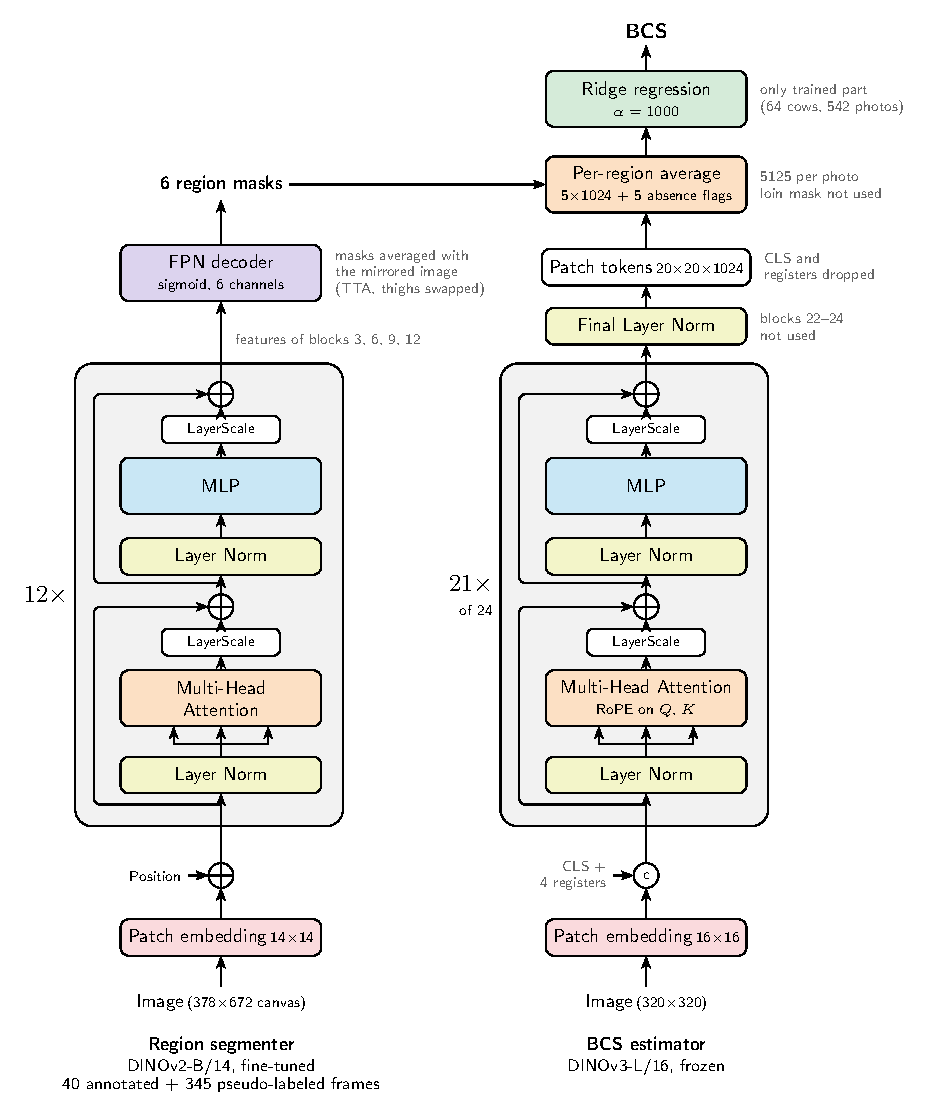
\includegraphics[width=\linewidth]{../figures/model_bcs_v3.pdf}
  \caption{BCS-Regions. Left: region segmenter (DINOv2-B/14 fine-tuned with an FPN decoder, mirror test-time augmentation). Right: frozen DINOv3-L/16 at 320\,px; tokens of block 21 of 24 are averaged inside five regions (all but the loin) and mapped to BCS by ridge regression. Only the ridge is fitted to BCS labels.}
  \label{fig:model}
\end{figure}

\subsubsection{Finding the regions a scorer looks at}

The first step locates six regions in the image: loin, hips, rump, tailhead, left thigh and right thigh.
These regions are not a partition of the cow's back.
The rump meets the thighs and the hips meet the thighs, and those meeting points are exactly the landmarks a scorer checks, so we let the regions overlap and treat segmentation as six independent binary problems rather than one multi-class one.

For this we fine-tuned a DINOv2-B/14 encoder \citep{oquab2024dinov2} with a feature pyramid decoder \citep{lin2017fpn}.
The decoder reads the encoder after blocks 3, 6, 9 and 12, projects each level to 128 channels with a $1\times1$ convolution and merges them top-down by bilinear upsampling; the concatenated pyramid then passes through a $3\times3$ convolution, batch normalisation and ReLU, and a final $1\times1$ convolution yields one sigmoid map per region.

Annotating regions is slow, so we started from only 40 full robot frames annotated in Roboflow (Fig.~\ref{fig:annotation}) and enlarged that set with pseudo-labels.

\begin{figure*}[t]
  \centering
  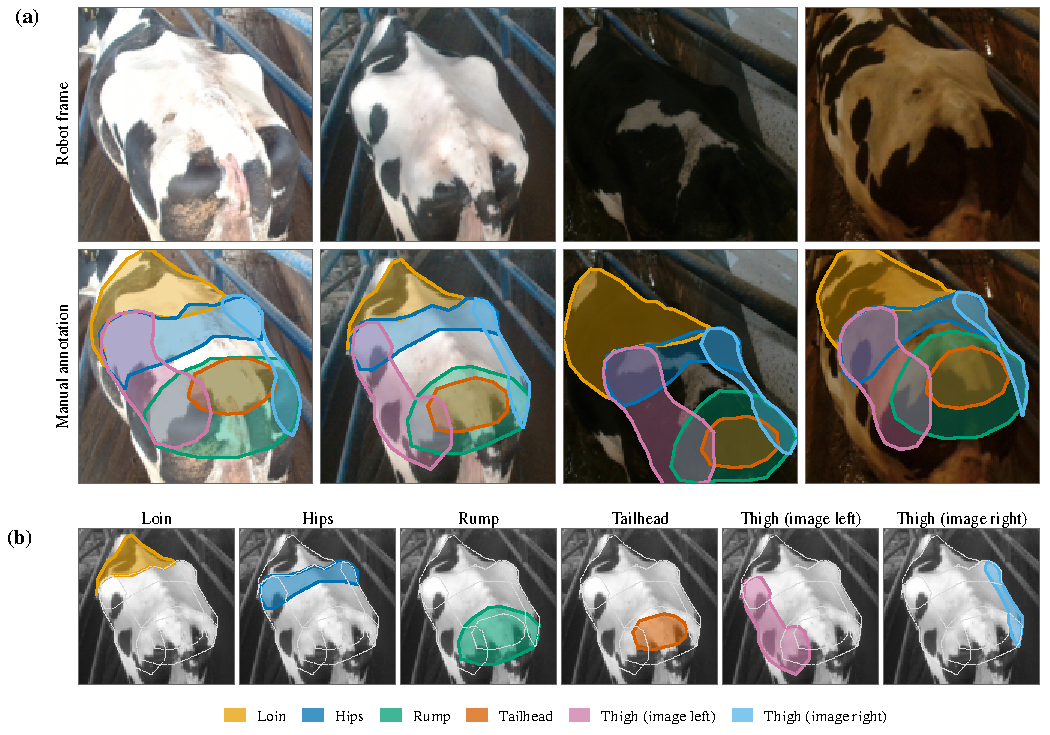
\includegraphics[width=\textwidth]{../figures/segmentation_examples.pdf}
  \caption{Manual region annotations on robot frames. (a) Four examples. (b) One frame, region by region.}
  \label{fig:annotation}
\end{figure*}
A first network (the teacher), trained on the 40 frames, labelled 493 unannotated frames, after excluding any frame taken within 10\,min of an annotated one so that near-copies could not leak into the training set.
We trusted the teacher only where it was consistent: we kept the 70\% of frames on which its prediction best agreed with its prediction on the mirrored image (345 frames, agreement mIoU 0.94), and ignored pixels with uncertain probability ($0.3 < p < 0.7$).
A second network (the student) was then trained with each batch split evenly between annotated and pseudo-labelled frames.
Both networks see full frames at $378\times672$\,px and are trained with binary cross-entropy plus Dice loss, batch 4 and learning rate $3\times10^{-4}$ (the encoder at one tenth of it), for 2000 iterations (teacher) and 3000 iterations (student).
In five-fold cross-validation on the annotated frames, the student reached mIoU 0.741, against 0.735 for the teacher recipe alone.

Since the segmenter was trained on full 16:9 frames while the BCS images are crops, we centre each crop on a 16:9 canvas filled with the ImageNet mean colour before segmenting it.
The cow then appears at the scale seen in training, and the resulting masks agree with those computed on the original frames (IoU 0.92).
At inference we also segment the mirrored image, swap its left and right thigh maps back, average both predictions and threshold at $p > 0.5$.

\pendiente{Check that no BCS image comes from the 40 annotated or 345 pseudo-labelled frames, or state it if some do.}

\subsubsection{Describing each region with a frozen foundation model}

With the regions located, the next question is what to measure inside them.
Hand-crafted cues such as depth or contour curvature require calibrated cameras and are fragile under the lighting of the exit lane; instead, we let a large self-supervised vision model describe the appearance of each region and keep that model frozen, so that no part of it is fitted to our few labels.

We use DINOv3 ViT-L/16 \citep{simeoni2025dinov3} (timm \texttt{vit\_large\_patch16\_dinov3.lvd1689m}, pretrained without labels on LVD-1689M), with rotary position embeddings \citep{su2024roformer}, one class token plus four register tokens \citep{darcet2024registers} and LayerScale \citep{touvron2021cait}.
Each crop is resized to $320\times320$\,px and normalised with ImageNet statistics, so the network produces a $20\times20$ grid of patch tokens, each a 1024-dimensional vector describing a $16\times16$-pixel patch of the cow.
We read these tokens after block 21 of 24, passed through the network's final LayerNorm, rather than at the output. The backbone and block were chosen in earlier experiments on this dataset; the resolution and the set of regions were chosen by the nested selection described in Sec.~\ref{sec:selection}.

The masks and the tokens now meet.
We resize each region mask to $320\times320$ and average it over every patch, which gives $w_{rp}$, the fraction of patch $p$ that lies in region $r$.
The description of region $r$ is then the average of the patch tokens $\mathbf{t}_p$, weighted by how much of each patch belongs to the region:
\begin{equation}
  \mathbf{v}_r = \frac{\sum_p w_{rp}\, \mathbf{t}_p}{\sum_p w_{rp}} .
  \label{eq:pool}
\end{equation}
A region may fall partly or wholly outside a crop.
When it covers less than half a patch in total ($\sum_p w_{rp} < 0.5$), we set $\mathbf{v}_r$ to zero and raise an absence flag, so that the regressor can tell a missing region from a real one.
The segmenter still delineates all six regions, but the descriptor keeps five: the loin, which lies outside the overlaps between bony landmarks, added noise rather than signal (Sec.~\ref{sec:selection}). Concatenating the five region vectors and their five flags gives a descriptor of $5\times1024 + 5 = 5125$ values per image.


\subsubsection{From descriptors to a score}

The last step is the only one that sees BCS labels, and we keep it as simple as possible: a ridge regression from the 5125-value descriptor to BCS.
A linear map has few degrees of freedom to overfit 64 cows, and its closed-form solution makes every fit deterministic.

Within each training set we standardise every column with the training mean and standard deviation.
With about 430 training images and 5125 features, it is far cheaper to solve the ridge in its dual form, through the $n\times n$ Gram matrix of the images:
\begin{equation}
  \hat{\mathbf{y}} = \bar{y} + \mathbf{X}_{\text{te}} \mathbf{X}^{\top} \left( \mathbf{X}\mathbf{X}^{\top} + \alpha \mathbf{I} \right)^{-1} (\mathbf{y} - \bar{y}) .
  \label{eq:ridge}
\end{equation}
One eigendecomposition of $\mathbf{X}\mathbf{X}^{\top}$ serves every candidate penalty $\alpha \in \{1, 10, 10^2, 10^3, 10^4, 10^5\}$.
We choose $\alpha$ by an inner four-fold cross-validation grouped by cow, run only on the training cows, keeping the value with the lowest mean absolute error; on all 64 cows this choice is $\alpha = 1000$.
The model outputs a continuous score.
Where a score on the 0.25 grid is needed, we round it to the nearest 0.25 and clip it to $[2.0, 5.0]$.

\subsection{Evaluation without identity leakage}
\label{sec:evaluation}

A model that has seen a cow during training can recognise her in the test set and recall her score instead of reading her body condition.
Images of the same cow taken minutes apart are close to duplicates, so this shortcut is easy to learn, and it would inflate any result obtained by splitting the data by image.
We therefore split every evaluation by cow: all images of a test cow are absent from training, from feature standardisation and from the choice of $\alpha$.

We use two schemes.
Leave-one-cow-out (LOCO) trains on 63 cows and tests on the remaining one, 64 times.
Because a single partition can be lucky, we also run five folds grouped by cow and stratified by BCS rounded to the nearest 0.5 (scikit-learn \texttt{StratifiedGroupKFold}), repeated with 10 random seeds, and average each image's prediction over the 10 repetitions before scoring.
As a reference floor, the same splits are scored by a model that always predicts the mean BCS of the training cows.

We report the usual image-level errors (mean absolute error, MAE, and root mean squared error, RMSE), $R^2$ over images and over cows (each cow's mean prediction against her mean label), and the share of images whose rounded prediction lies within 0.5 points of the label.
Our main metric, however, is the MAE per cow: the mean, over cows, of each cow's MAE.
It gives every cow the same weight regardless of how often she was photographed, which is the quantity a farm cares about.
Its 95\% confidence interval comes from 5000 bootstrap resamples of the cows.
To compare two methods, we compute the per-cow difference in MAE on identical splits and bootstrap it over cows; we call the difference significant when its 95\% interval excludes zero.

\subsection{Choosing the final configuration without selection bias}
\label{sec:selection}

Two changes to an earlier version of the model looked promising on these same cows: dropping the loin from the descriptor, and describing the image at 320 instead of 384\,px.
Choosing between them by their cross-validated error would reuse the test cows for a decision, and the reported error would then be optimistic.
We therefore made the choice inside the cross-validation itself.
For each outer fold (both schemes above), the four combinations of \{six regions, five regions without the loin\} and \{384, 320\,px\} were compared by a five-fold grouped cross-validation on the training cows only, and the one with the lowest MAE per cow was retrained on all training cows to predict the held-out cows.
The previous model was kept unless another configuration was strictly better, and the design was written down before any result was computed.
A second round, starting from the selected configuration, tried ten further variants in the same way: 288 and 256\,px, blocks 19, 20, 22 and 23, a greyscale image, two ways of combining 320 and 384\,px, and removing the descriptor directions that separate cows without predicting their score.

\pendiente{The candidate changes were proposed after looking at results on these 64 cows; nested selection corrects the choice among them but not their proposal. A held-out set of new cows is needed for a fully independent confirmation.}

\subsection{Additional analyses}
\label{sec:analyses}

Beyond the overall error, three analyses describe how the model behaves; all use the leave-one-cow-out predictions.
First, we report error and bias for each BCS value and a Bland--Altman analysis \citep{bland1986} of the mean prediction for each cow and score.
Second, for cows photographed on several days without a change of score, we measured how much the daily mean prediction varies, and we followed the two cows whose score changed during the study.
Third, a learning curve trained the model on random subsets of 8 to 56 cows, with eight cows always held out for testing (10 repetitions), to estimate how much more data would help.
Finally, to test whether the anatomical regions matter, we replaced the region descriptor by simpler ones built from the same tokens: the class token and mean of all patches of the whole image, the mean of the patches inside the cow's silhouette (the union of all six masks), and a single rectangular crop of the rear, which mimics single-crop methods \citep{nagy2023}.


\subsection{Baselines and leakage experiment}
\label{sec:baselines}

To place BCS-Regions against the usual alternative, end-to-end fine-tuning of an image network, we trained eight 2D, image-only baselines (Table~\ref{tab:baselines}) on exactly the same cow-level splits, using the first 3 seeds of the repeated five-fold scheme (15 folds).
All of them receive the whole crop resized to $384\times384$\,px with ImageNet normalisation, the native or usual input size of these networks.
Three are convolutional regressors fine-tuned in full (ResNet-50, EfficientNet-B0 and EfficientNet-V2, the last used for BCS by \citet{siachos2023}), and a fourth is a supervised vision transformer, as in transformer-based BCS work \citep{vitbcs2021}.
The third asks whether our frozen backbone would do better if adapted: it fine-tunes the same DINOv3 model with low-rank adapters \citep{hu2022lora} and a linear head.
Two follow published work that classifies BCS with YOLO, in the version used in most papers (YOLOv8) and the current one (YOLO11), and the last, a frozen ResNet-50 with our ridge head, isolates the contribution of the foundation model.

\begin{table*}[t]
  \centering
  \caption{Baselines. All use the same cow-level splits and input as the proposed model.}
  \label{tab:baselines}
  \begin{tabular}{llll}
    \toprule
    Baseline & Backbone (pretraining) & Trained & Output \\
    \midrule
    ResNet-50, fine-tuned & ResNet-50 \citep{he2016resnet} (timm a1, ImageNet-1k) & all weights & regression \\
    EfficientNet-B0, fine-tuned & EfficientNet-B0 \citep{tan2019efficientnet} (timm ra, ImageNet-1k) & all weights & regression \\
    EfficientNet-V2-S, fine-tuned & EfficientNet-V2-S \citep{tan2021efficientnetv2} (timm tf, ImageNet-1k) & all weights & regression \\
    ViT-B/16, fine-tuned & DeiT-B/16 at 384\,px \citep{touvron2021deit} (ImageNet-1k) & all weights & regression \\
    DINOv3 + LoRA & DINOv3 ViT-L/16, as in the model & LoRA $r=8$ on qkv and projection, 24 blocks; linear head & regression \\
    YOLOv8s-cls & YOLOv8s-cls \citep{jocher2023yolov8} (ImageNet) & all weights & classes = BCS values \\
    YOLO11s-cls & YOLO11s-cls \citep{jocher2024yolo11} (ImageNet) & all weights & classes = BCS values \\
    ResNet-50, frozen & ResNet-50 (as above) & ridge on 2048 pooled features & regression \\
    \bottomrule
  \end{tabular}
\end{table*}

The fine-tuned regressors predict BCS standardised with the training mean and standard deviation, with a SmoothL1 loss, AdamW \citep{loshchilov2019adamw} (weight decay 0.05), one warm-up epoch followed by cosine decay, and mixed precision.
They are trained with horizontal flips, mild affine transforms ($\pm10^\circ$, $\pm5\%$ shift, scale 0.9--1.1) and colour jitter (brightness and contrast 0.2, saturation 0.1).
ResNet-50 is tried with learning rates $\{10^{-4}, 3\times10^{-4}, 10^{-3}\}$ and EfficientNet-B0 and EfficientNet-V2-S with $\{3\times10^{-4}, 10^{-3}\}$, all for 30 epochs with batch 16; the ViT-B/16 with $\{3\times10^{-5}, 10^{-4}\}$ for 15 epochs with batch 8 and gradient checkpointing; DINOv3 with LoRA is tried with $\{3\times10^{-4}, 10^{-3}\}$ for 15 epochs with batch 8 and gradient checkpointing.

These networks have many more hyperparameters than our ridge, and choosing them on the test cows would favour them unfairly.
Inside each outer training set, we hold out 20\% of the cows for validation.
With so few cows a random 20\% can be badly skewed (for example, only fat cows), so among 30 random cow-level splits we use the one whose BCS mean and standard deviation best match the training set.
For each learning rate we keep the epoch with the lowest validation MAE, and the learning rate with the lowest validation MAE then predicts the outer test fold.
Both YOLO classifiers are trained on the same split following the standard Ultralytics practice (30 epochs, best checkpoint by validation accuracy), and its continuous prediction is the expected value of BCS under its class probabilities.

Finally, to measure how much an image-level split inflates the results, we re-run the proposed model, both ResNet-50 variants and YOLOv8s-cls with a plain five-fold split by image (\texttt{StratifiedKFold}, 3 seeds), in which images of one cow fall in both training and test.
The gap between the two splits measures the identity leakage discussed above.

\pendiente{Cite the published 2D BCS methods each baseline stands for (e.g.\ YOLO classifiers such as Dand\i l et al.).}

\subsection{Implementation and reproducibility}
\label{sec:implementation}

Because the segmenter and the backbone are fixed, masks and descriptors are computed once per image, and each evaluation fold only refits the ridge, which takes seconds.
Fine-tuning DINOv3 with LoRA, by contrast, takes about 1.2\,h per seed of five folds on the same GPU.
The code uses PyTorch 2.9.1 (CUDA 12.6), timm 1.0.22 \citep{wightman2019timm}, NumPy 2.2.6, scikit-learn and, for the YOLO baseline only, Ultralytics 8.3.150, and it runs in Docker containers built from the repository.
Every cached result (masks, descriptors, fitted ridge) records the backbone, input size, block, region list and MD5 of the segmenter weights that produced it, and the pipeline stops if these do not match the current code.
The segmenter weights are published as a GitHub release (\texttt{bcs-regions-v2}), and the code is available at \url{https://github.com/MonicaMMartinezV/MuuMetrics}.

\pendiente{GPU model for the timing figures; end-to-end runtime of the proposed model.}
\pendiente{Data availability statement (images and labels public or on request).}

% =============================================================
% Results (draft) -- BCS-Regions paper, canonical model v3 (320 px, five regions)
% Numbers: work/metrics.csv (model/main, EXPERIMENTOS [32]); selection [30] (model/mejoras);
% baselines and leakage [28] (model/baselines, work/baselines/comparacion.csv);
% analyses and region ablation [31] (model/ablations, work/analisis/, work/exp_curva/).
% =============================================================
\section{Results}
\label{sec:results}

\subsection{Accuracy on unseen cows}

Evaluated on cows it had never seen, BCS-Regions estimated body condition with a mean absolute error of 0.431 points under leave-one-cow-out (RMSE 0.542; $R^2 = 0.71$ over images and 0.68 over cows; Pearson $r = 0.85$).
For 75\% of the images, the prediction rounded to the 0.25 grid fell within 0.5 points of the reference score.
Weighting every cow equally, the MAE per cow was 0.427 (95\% CI 0.367--0.492).
The repeated five-fold scheme, which holds out a fifth of the herd at a time, gave almost the same figures (MAE 0.442, MAE per cow 0.434, 95\% CI 0.374--0.498), and the error varied little across the 10 random partitions (SD 0.022).

\subsection{Choice of the final configuration}

When the configuration was chosen inside each training set, as described in Sec.~\ref{sec:selection}, the inner validation picked 320\,px with five regions in 57 of the 64 leave-one-cow-out folds and in 32 of the 50 repeated five-fold folds (Table~\ref{tab:selection}).
This nested procedure, which never saw the test cows when choosing, lowered the MAE per cow by 0.021 points (95\% CI 0.003--0.039) with respect to the previous model, and by 0.019 (0.005--0.032) in the repeated scheme.
The two changes added up: each alone gained about 0.01, and together 0.026.
In the second round, none of the ten further variants improved on this configuration, and choosing among all eleven by inner validation made the error worse (+0.016 per cow), the expected cost of selecting among many near-equivalent options.
We therefore took 320\,px with five regions as the final model.

\begin{table}[t]
  \centering
  \caption{Selection of the final configuration (leave-one-cow-out). $\Delta$: MAE per cow minus that of the previous model (384\,px, six regions), paired bootstrap 95\% CI over cows. Nested: configuration chosen inside each training set.}
  \label{tab:selection}
  \begin{tabular}{lccc}
    \toprule
    Configuration & MAE/cow & $r$ & $\Delta$ MAE/cow [95\% CI] \\
    \midrule
    384\,px, six regions (previous) & 0.452 & 0.830 & -- \\
    384\,px, without loin & 0.440 & 0.837 & $-$0.012 [$-$0.023, $-$0.001] \\
    320\,px, six regions & 0.439 & 0.840 & $-$0.013 [$-$0.029, +0.001] \\
    320\,px, without loin (final) & \textbf{0.427} & \textbf{0.846} & $-$0.026 [$-$0.043, $-$0.008] \\
    Nested selection & 0.432 & 0.844 & $-$0.021 [$-$0.039, $-$0.003] \\
    \bottomrule
  \end{tabular}
\end{table}

\subsection{Do the anatomical regions matter?}

Describing the cow by regions was clearly better than describing the image as a whole (Table~\ref{tab:regions}).
Averaging the same tokens over the whole image raised the MAE per cow by 0.080, and a single crop of the rear, as in single-crop methods, by 0.109.
Most of the gain came from locating the cow, but splitting her into regions also helped: the mean over her silhouette was 0.039 points worse per cow than the five regions (95\% CI 0.011--0.070).
Adding the whole-image descriptor to the regions made the model slightly worse (+0.011), so the background carries no useful information.

\begin{table}[t]
  \centering
  \caption{Region descriptor against simpler descriptors built from the same frozen tokens (leave-one-cow-out). $\Delta$: MAE per cow minus that of the five regions, paired bootstrap 95\% CI over cows.}
  \label{tab:regions}
  \begin{tabular}{lccc}
    \toprule
    Descriptor & Dim. & MAE/cow & $\Delta$ MAE/cow [95\% CI] \\
    \midrule
    Five regions (model) & 5125 & \textbf{0.427} & -- \\
    Silhouette (union of masks) & 1024 & 0.469 & +0.039 [+0.011, +0.070] \\
    Whole image (CLS + mean) & 2048 & 0.519 & +0.080 [+0.041, +0.120] \\
    Rear crop (CLS + mean) & 2048 & 0.545 & +0.109 [+0.066, +0.153] \\
    Regions + whole image & 7173 & 0.438 & +0.011 [+0.001, +0.022] \\
    \bottomrule
  \end{tabular}
\end{table}

\pendiente{The final region set came out of the selection on these cows while the silhouette had no selection; part of the +0.039 may be optimistic.}

\subsection{Comparison with end-to-end networks}

Table~\ref{tab:baselines-results} places BCS-Regions against the baselines on the same 15 cow-level folds; the model's figures differ slightly from the first subsection because only 3 of the 10 partitions are used.

\begin{table*}[t]
  \centering
  \caption{BCS-Regions against the baselines, split by cow (15 folds: five folds $\times$ 3 seeds; each image's prediction averaged over the seeds). $\Delta$: per-cow MAE of the baseline minus that of BCS-Regions, with a paired bootstrap 95\% CI over cows; positive means the baseline is worse. Bias: mean signed error for thin ($<3$) and fat ($\geq4.5$) cows.}
  \label{tab:baselines-results}
  \begin{tabular}{lcccccccc}
    \toprule
    Method & MAE & RMSE & $R^2$ & $\pm0.5$ & MAE/cow & $\Delta$ MAE/cow [95\% CI] & Bias thin & Bias fat \\
    \midrule
    BCS-Regions & \textbf{0.458} & \textbf{0.565} & \textbf{0.68} & \textbf{73\%} & \textbf{0.443} & -- & \textbf{+0.61} & \textbf{$-$0.36} \\
    DINOv3 + LoRA & 0.505 & 0.639 & 0.59 & 68\% & 0.455 & +0.012 [$-$0.037, +0.057] & +0.70 & $-$0.42 \\
    ResNet-50, frozen + ridge & 0.676 & 0.840 & 0.29 & 52\% & 0.656 & +0.213 [+0.138, +0.289] & +0.86 & $-$0.74 \\
    ResNet-50, fine-tuned & 0.726 & 0.880 & 0.22 & 47\% & 0.650 & +0.207 [+0.132, +0.282] & +1.10 & $-$0.70 \\
    EfficientNet-B0, fine-tuned & 0.766 & 0.907 & 0.17 & 44\% & 0.687 & +0.243 [+0.169, +0.319] & +1.22 & $-$0.72 \\
    YOLOv8s-cls & 0.801 & 0.946 & 0.10 & 44\% & 0.701 & +0.258 [+0.167, +0.347] & +1.19 & $-$0.78 \\
    \bottomrule
  \end{tabular}
\end{table*}

\pendiente{Add the rows of EfficientNet-V2-S, ViT-B/16 and YOLO11s-cls when their runs finish.}

The networks most often used for BCS in the literature fell well behind.
The fine-tuned convolutional networks and the YOLOv8 classifier made errors 0.21 to 0.26 points per cow larger than BCS-Regions, and all confidence intervals exclude zero.
Their $R^2$ over images stayed between 0.10 and 0.22, so they explained little of the variation in body condition among new cows.
A frozen ResNet-50 with our ridge head did no better than the fine-tuned one (0.656 against 0.650 per cow): with the head fixed, the gap from 0.656 to 0.443 comes from the representation.

Only fine-tuning the same foundation model came close.
DINOv3 adapted with LoRA had a higher error per image (0.505 against 0.458), a lower $R^2$ (0.59 against 0.68) and a slightly higher error per cow (0.455 against 0.443), a difference that was not significant.
The averaged predictions in Table~\ref{tab:baselines-results} even favour LoRA, since averaging over seeds turns its three trained networks into an ensemble while it barely changes a ridge fit; seed by seed, BCS-Regions had the lower error in all three seeds, per image (0.469, 0.475, 0.456 against 0.579, 0.535, 0.498) and per cow (0.457, 0.451, 0.450 against 0.511, 0.489, 0.459; mean advantage 0.034, 95\% CI $-$0.013 to 0.078).
The two approaches are therefore at least equivalent in accuracy, but not in cost: LoRA needed about 4.8\,h of GPU training for the three seeds and its error moved from 0.498 to 0.579 with the seed, whereas BCS-Regions computes each descriptor once and refits a ridge in seconds, with a deterministic result.

\subsection{The cost of splitting by image}

Splitting the same data by image instead of by cow changed the picture completely (Table~\ref{tab:leakage}).
Every method appeared two to three times more accurate, and the ranking between them almost disappeared.

\begin{table}[t]
  \centering
  \caption{Effect of identity leakage. Same methods and seeds, with five folds split by cow (no cow in both training and test) or by image (images of one cow in both).}
  \label{tab:leakage}
  \begin{tabular}{lcccc}
    \toprule
    & \multicolumn{2}{c}{MAE} & \multicolumn{2}{c}{$\pm0.5$} \\
    \cmidrule(lr){2-3}\cmidrule(lr){4-5}
    Method & by cow & by image & by cow & by image \\
    \midrule
    BCS-Regions & 0.458 & 0.249 & 73\% & 92\% \\
    ResNet-50, fine-tuned & 0.726 & 0.253 & 47\% & 89\% \\
    YOLOv8s-cls & 0.801 & 0.244 & 44\% & 88\% \\
    ResNet-50, frozen + ridge & 0.676 & 0.442 & 52\% & 76\% \\
    \bottomrule
  \end{tabular}
\end{table}

The YOLOv8 classifier, the weakest method on unseen cows (MAE 0.801), became as accurate as BCS-Regions once its test cows were also in training (0.244 against 0.249), and so did the fine-tuned ResNet-50 (0.253).
Under this split neither was significantly worse than BCS-Regions per cow (+0.057, 95\% CI $-$0.006 to +0.124; +0.029, $-$0.019 to +0.078).
A network trained end to end can recognise a cow it has already seen and return her score, and the image split rewards exactly that; the frozen ResNet-50, which can only fit a linear map, benefited much less (0.676 to 0.442).
Results obtained with image-level splits therefore say little about how a model will score the next cow that enters the robot, and they can hide large differences between methods.

\subsection{Where the model errs}

The overall bias was close to zero ($-$0.04 points), but the errors depended on the level of body condition (Fig.~\ref{fig:ba}).
Predictions were compressed toward the herd mean: the slope of predicted against reference score was 0.60, so thin cows were overestimated (+0.45 to +0.73 points between BCS 2.0 and 2.75) and fat cows underestimated ($-$0.19 to $-$0.39 between 4.0 and 5.0).
The model was most accurate between 3.5 and 4.25, where the MAE per cow was 0.25--0.34.
For the mean prediction of each cow and score, the 95\% limits of agreement were $-$0.98 to +0.89, and 66\% of these means fell within 0.5 points of the reference.

\begin{figure*}[t]
  \centering
  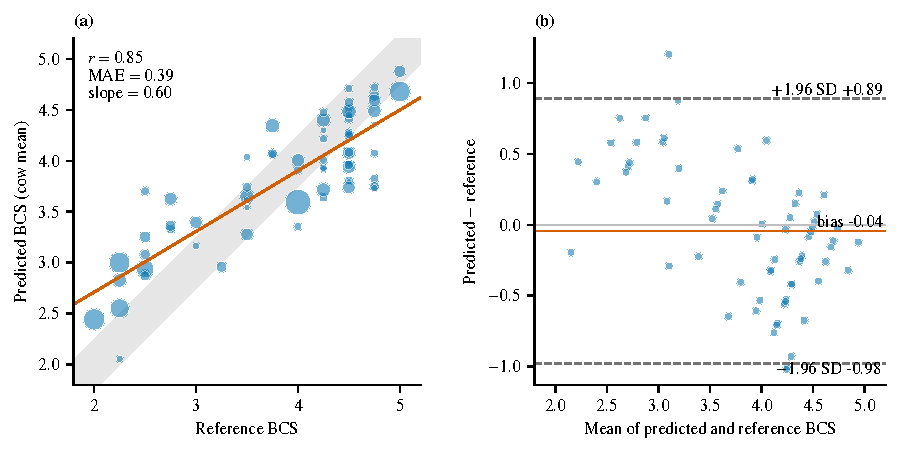
\includegraphics[width=\textwidth]{../figures/analisis_bland_altman.pdf}
  \caption{Agreement with the reference score (leave-one-cow-out; one point per cow and score, size proportional to the number of images). (a) Predicted against reference BCS; dashed: identity, grey band: $\pm0.25$, orange: least-squares fit. (b) Bland--Altman plot; orange: mean difference, dashed: 95\% limits of agreement.}
  \label{fig:ba}
\end{figure*}

\subsection{Stability over time and sample size}

Predictions for a given cow were stable from day to day.
For the 55 cow--score pairs photographed on at least two days, the daily mean prediction varied with a median SD of 0.23 points, less than the typical bias of each cow (0.42), and 86\% of the variance of the predictions lay between cows (intraclass correlation 0.86).
The error is therefore mostly a stable offset per cow rather than noise between photos, which is also why averaging more photos of the same cow helps little.
The model also followed real changes in condition (Fig.~\ref{fig:tracking}).
Cow 9008 fell ill and was rescored from 4.5 to 2.25 within a month; her predictions dropped from 4.15 at the start of the period to about 3.0--3.4 in early June, while she was still recorded as 4.5, and to 2.0 when she was rescored.
Cow 8758, scored 4.25, 4.0 and 3.5 in three months, was predicted at 3.92, 4.01 and 3.54.

\begin{figure}[t]
  \centering
  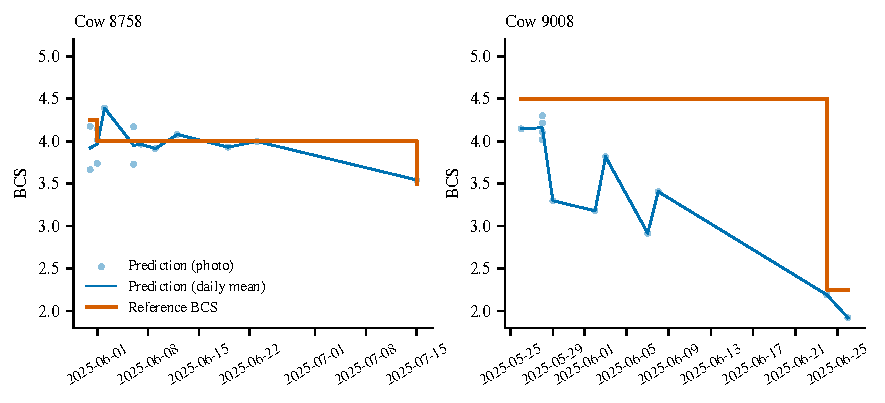
\includegraphics[width=\linewidth]{../figures/analisis_cambios_bcs.pdf}
  \caption{Predictions (leave-one-cow-out) for the two cows whose score changed during the study; orange: reference score.}
  \label{fig:tracking}
\end{figure}

Finally, the error kept falling as more cows were used for training: the MAE per cow went from 0.69 with 8 cows to 0.57 with 16, 0.48 with 32 and 0.44 with 56, while the bias for thin cows fell from +0.99 to +0.55.
A fit of the form $a + b/\sqrt{n}$ to the MAE per cow suggests about 0.40 with 100 cows and 0.37 with 200 (Fig.~\ref{fig:curve}), an extrapolation that assumes new cows resemble the present ones.

\begin{figure*}[t]
  \centering
  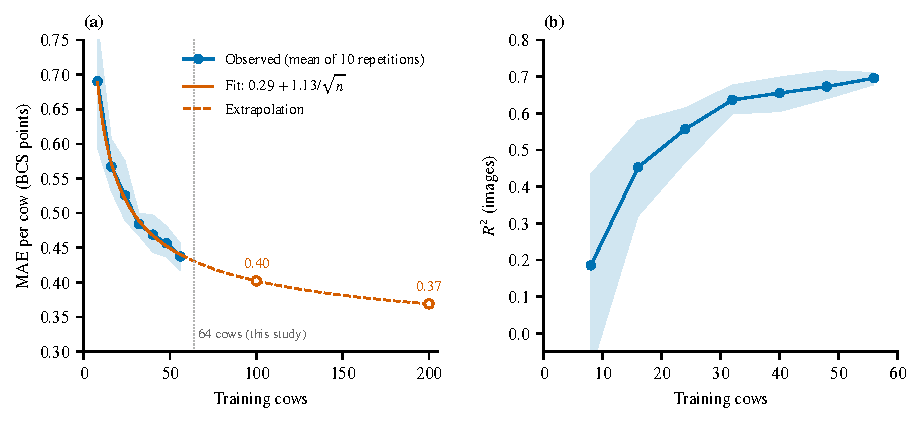
\includegraphics[width=\textwidth]{../figures/curva_aprendizaje.pdf}
  \caption{Learning curve. The model was trained on random subsets of $n$ cows and tested on eight held-out cows (8 folds $\times$ 10 repetitions). (a) MAE per cow; band: 2.5--97.5 percentiles over repetitions; orange: fit $a + b/\sqrt{n}$ and its extrapolation. (b) $R^2$ over images.}
  \label{fig:curve}
\end{figure*}


\bibliographystyle{plainnat}
\bibliography{refs}
\end{document}
